\chapter{Goldprobe}
%Alle mit dem RTM aufgenommenen Bilder wurden mithilfe der frei verfügbaren Software „Gwyddion“ nachbearbeitet.
%Die Software ermöglicht eine Vielzahl von Bildbearbeitungsfunktionen, darunter Rauschunterdrückung, Filterung und Kontrastanpassung. Diese Schritte sind entscheidend, um die Qualität der Bilder zu verbessern und die atomaren Strukturen klarer darzustellen.\\
%Im ersten Versuchsteil wird eine Goldkugelprobe untersucht. Um die Leitfähigkeit von der Probe sicherzustellen, wurde Gold auf Silizium aufgedampft. Die Oberfläche wurde unter dem Mikroskop vergrößert (siehe Abbildung !!!!!!!ADD REFERENCE!!!!!!). 
%Das rechte Bild zeigt einen vergrößerten Ausschnitt des linken Bildes. Zu beachten ist, dass die verwendete Probe nicht völlig eben und kratzfrei ist. Für das Experiment stellt dies jedoch kein Problem dar, da genügend möglichst ebene und kratzfreie Bereiche vorhanden sind. Für diesen Teil des Experiments wurde die Spitze aus Abbildung !!!!!!!ADD REFERENCE!!!!!! verwendet.
%\begin{figure}[H]
 %   \centering
  %  \includegraphics[width=0.8\textwidth]{}
   % \caption{Goldkugelprobe unter dem Mikroskop. Links: Gesamtansicht, rechts: vergrößerter Ausschnitt.}
   % \label{fig:goldprobe}
%\end{figure}
%Die Messung wurde im Constant Current Mode durchgeführt, wobei eine Tunnelspannung von $U = 1\,\text{V}$ und ein Strom von $I = 1\,\text{nA}$ eingestellt wurden. Die PID-Regelparameter waren $P = 1000$, $I = 2000$ und $D = 0$. Der Scanbereich betrug $???,\text{nm} \times ???\text{nm}$. Das resultierende Bild zeigt die topografischen Eigenschaften der Goldprobe mit hoher lateraler und vertikaler Auflösung. Die atomaren Strukturen sind deutlich erkennbar, was auf die hohe Präzision des RTM hinweist.\\

%Die verarbeiteten Bilder sind in den Abbildungen !!!!!!!ADD REFERENCE!!!!!! dargestellt. Sie zeigen das Höhenprofil sowohl im 2D- als auch im 3D-Format, ergänzt durch die entsprechenden Strombilder.
%add the pictures taken with the microscope on different scales 

%Die theoretische Erwartung wurde durch die Untersuchung der Goldprobe bestätigt. Die Goldprobe weist keine regelmäßige Oberflächenstruktur auf. Dies entspricht den Erwartungen, da sich die Elektronen in Gold wie ein frei bewegliches Elektronengas (Fermigas) mit wolkenartiger Verteilung verhalten. Diese Eigenschaft ist typisch für Metalloberflächen, bei denen Elektronentransfer zu einer nahezu kontinuierlichen und homogenen Tunnelstromverteilung führt – im Gegensatz zur lokalen, geordneten Strukturen. Auffällig ist, dass die Elektronenverteilung in hellen Bereichen deutlich größer ist als in dunklen. Darüber hinaus ist klar, dass der PID-Regelkreis mit geeigneten Parametern arbeitet, da die Strombilder insgesamt einen geringen Kontrast aufweisen, was auf eine geringe Stromschwankung hindeutet. %verify this observation

%Die Bilder weisen möglichst wenige Fehler und Verzerrungen auf, die durch eine optimale PID-Regelung oder eine zu hohe Scangeschwindigkeit verursacht werden können. Im Experiment zeigte sich, dass langsameres Scannen zu einer höheren Auflösung der erfassten Struktur führte. Der Nachteil dieser Methode ist die längere Aufnahmezeit, die mögliche Bildfehler, beispielsweise durch Geräusche oder Bewegungen, verstärken kann. Daher ist die Wahl einer angemessenen Scangeschwindigkeit für die Messung entscheidend. Trotz der geringen Bildfehler kann festgestellt werden, dass die Bilder ihren Zweck erfüllen und eine repräsentative Darstellung der Goldprobe liefern.


Beide Goldproben werden aus dem verfügbaren Satz ausgewählt und anschließend untersucht wird. 
Da Beispiele für die Oberflächen von Gold auf Saphir und auf Silizium bekannt sind \cite{praktikum}, empfiehlt sich der ''Constant Current Mode'' (CCM), da die Spitze sonst bei Kontakt mit einer rauen Oberfläche brechen könnte.

\begin{figure}[H]
    \centering
    \begin{minipage}[t]{0.495\textwidth}
        \centering
        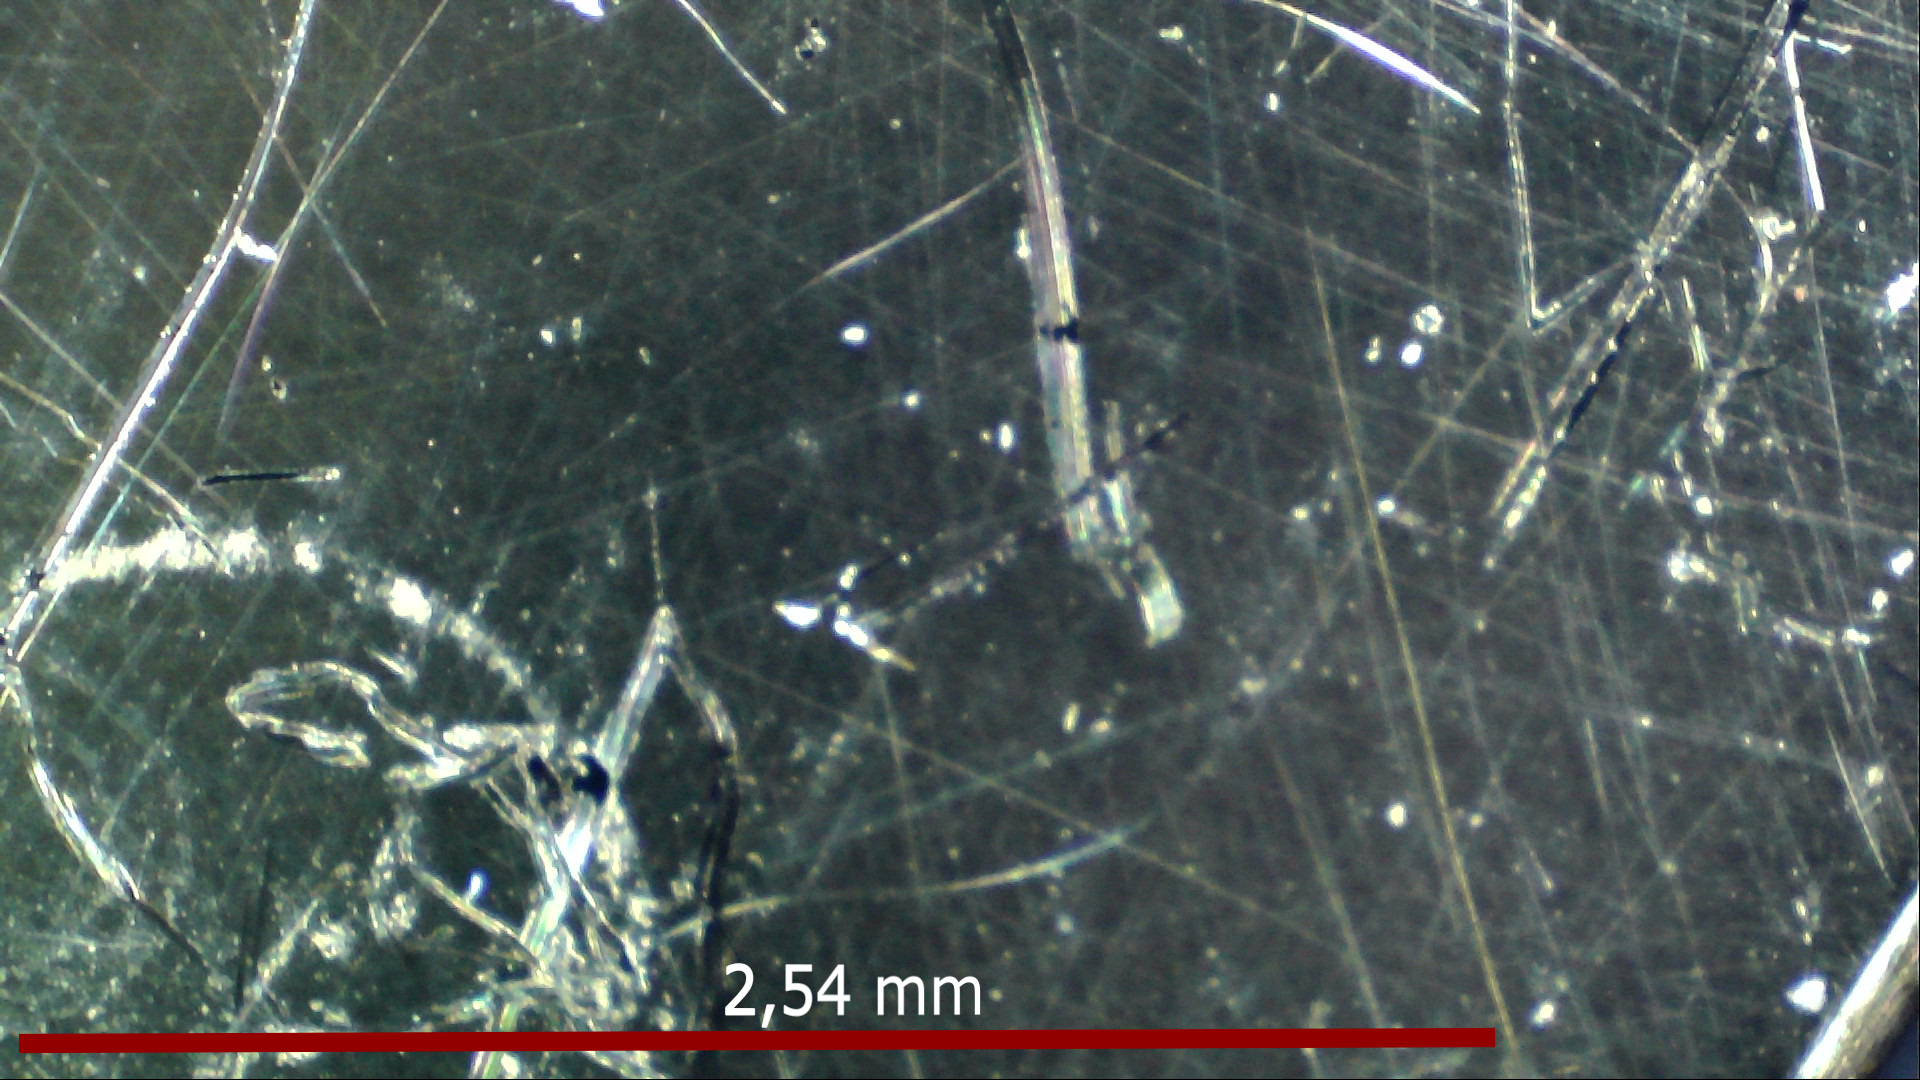
\includegraphics[width=\textwidth]{editgold_on_safir.png}
        \subcaption{Gold auf Saphir}
        \label{fig:golda}
    \end{minipage}
    \hfill
    \begin{minipage}[t]{0.495\textwidth}
        \centering
        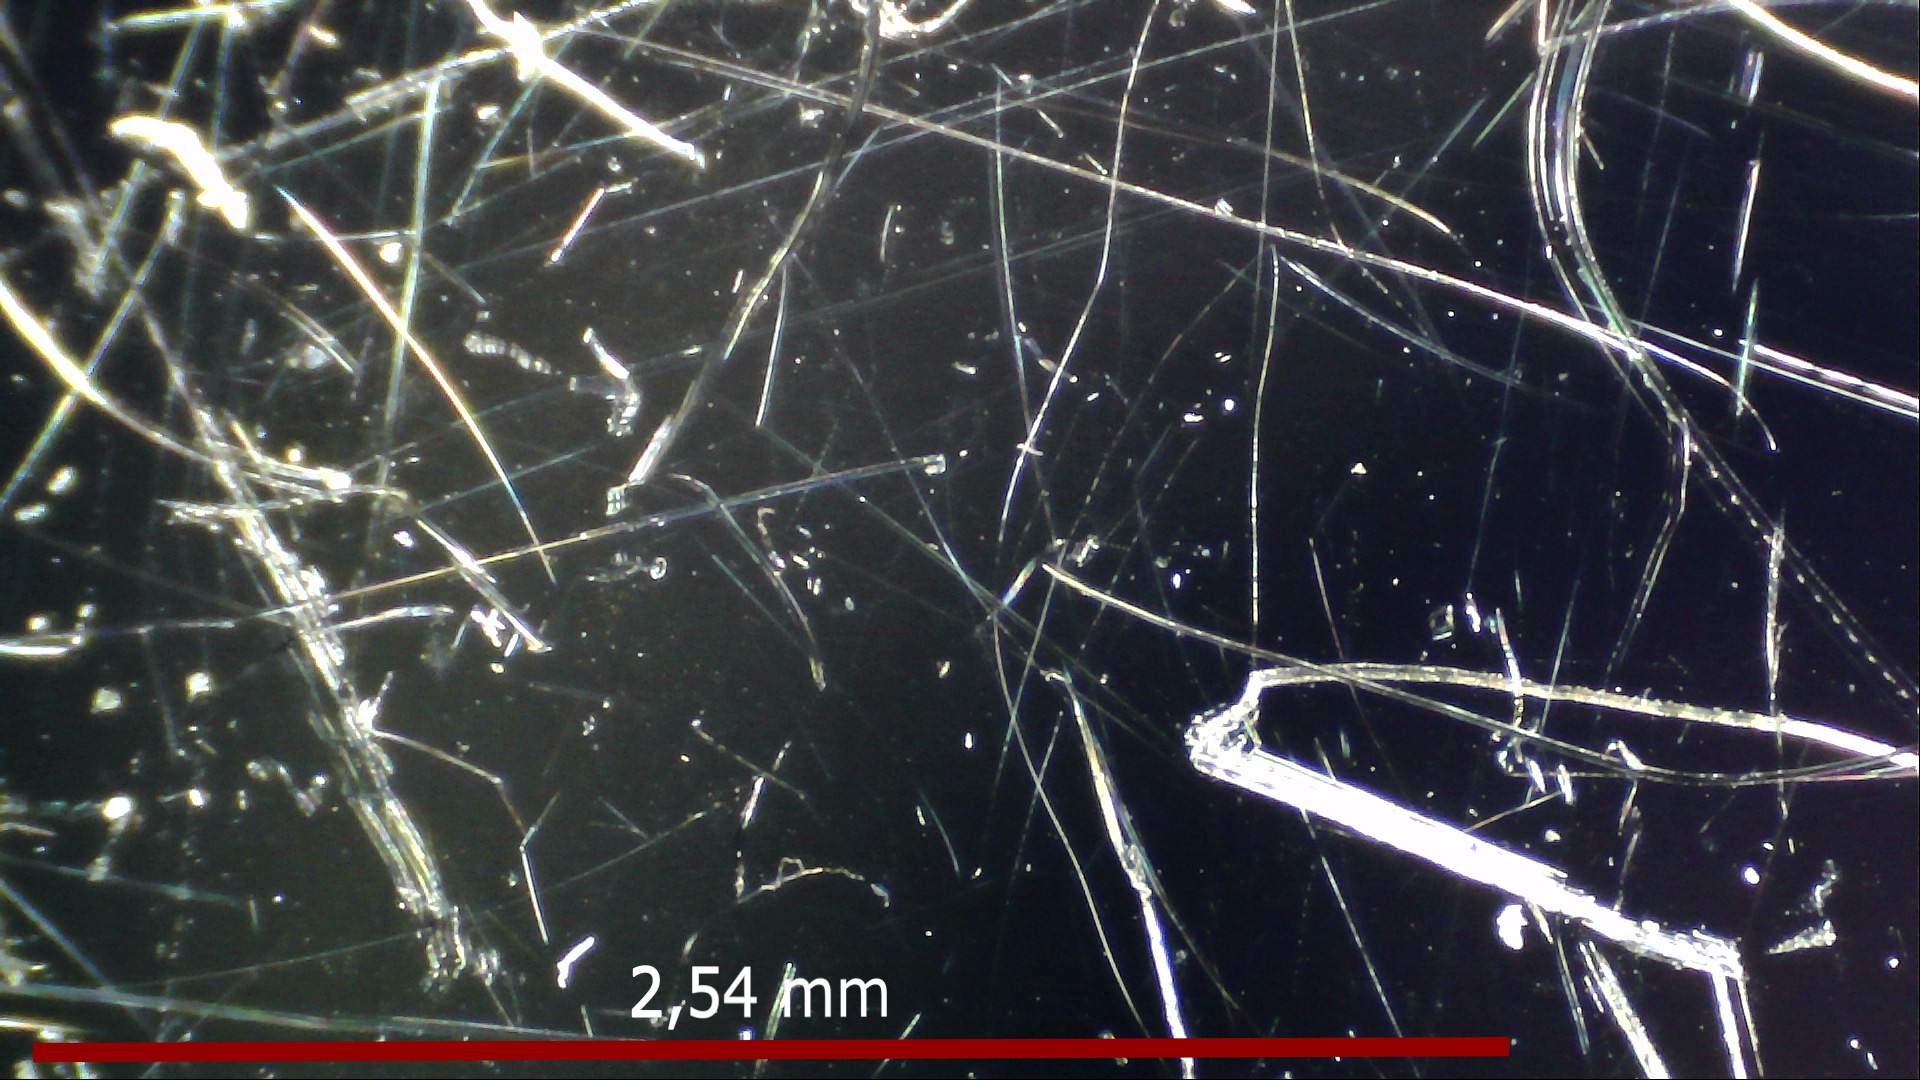
\includegraphics[width=\textwidth]{editgold_on_silizium.png}
        \subcaption{Gold auf Silizium}
        \label{fig:goldb}
    \end{minipage}
    \caption{Beide Goldproben unter dem USB-Mikroskop mit einer Linie der Länge $\SI{2.54}{\mm}$ als Maßstab.}
    \label{fig:gold_combined}
\end{figure}

Kratzer auf der Oberfläche lassen sich bereits in \cref{fig:gold_combined} mit dem USB-Mikroskop erkennen, deren Breite im Mikrometerbereich liegt. 
Sie stellen eine potenzielle Fehlerquelle dar: Kleinere Kratzer könnten so groß sein wie der künftige Bildausschnitt, weil das USB-Mikroskop nur die größten Kratzer erfasst. 
Wären die Kratzer größer, wäre dies kein Problem, da sie die lokal aufgezeichnete Struktur nicht beeinflussen würden. Ansonsten sind keine signifikanten Verunreinigungen oder zusätzlichen Oberflächenschäden feststellbar.

Nun beginnt die eigentliche Messung mit dem STM.
Die Spitze und die Probe werden in das STM eingesetzt, und zunächst wird ein Bild mit den Abmessungen $\SI{200}{\nm} \times \SI{200}{\nm}$ aufgenommen. 
Um die Scan-Geschwindigkeit zu berechnen, die einen Einfluss auf die Schärfe des aufgenommenen Bildes hat, muss die Bildlänge durch die vom Programm angegebene Geschwindigkeit dividiert werden. 
Dies ist darauf zurückzuführen, dass die vom Programm bereitgestellte Geschwindigkeit in ''Time per Line'' angegeben ist, also der Zeit, die die Spitze benötigt, um eine Scanzeile zu durchfahren (d.h. einen horizontalen Durchgang über den Bildausschnitt).

\begin{figure}[H]
    \centering
    \begin{minipage}[t]{0.495\textwidth}
        \centering
        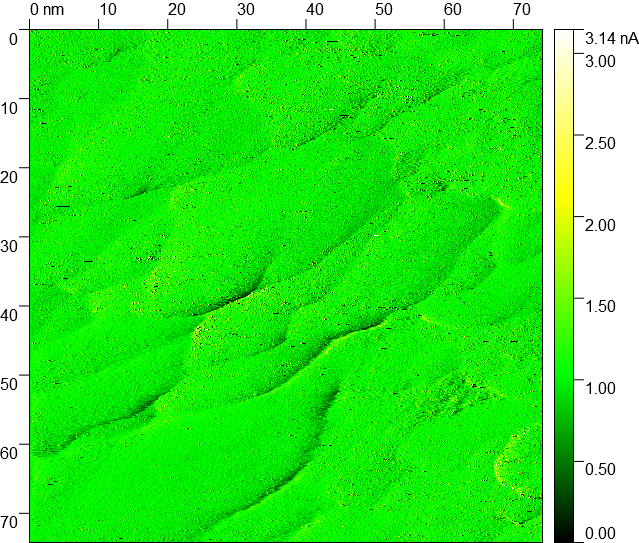
\includegraphics[width=\textwidth]{Au_Rund_useI.png}
        \label{fig:goldrund_I}
    \end{minipage}
    \hfill
    \begin{minipage}[t]{0.495\textwidth}
        \centering
        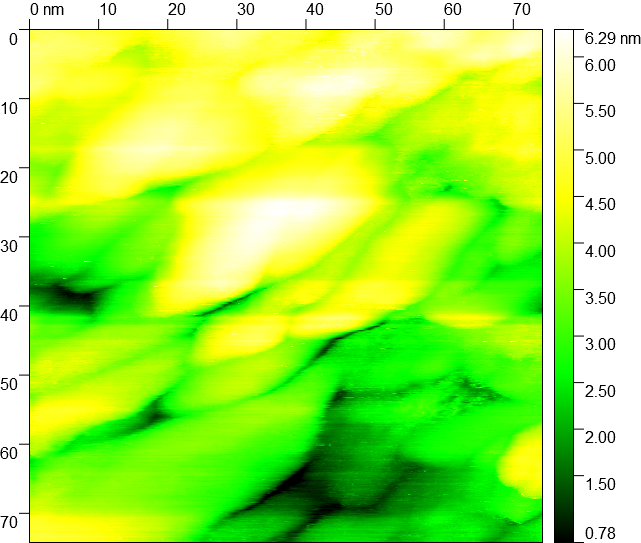
\includegraphics[width=\textwidth]{Au_Rund_useZ.png}
        \label{fig:goldrund_Z}
    \end{minipage}
    \caption{
      RTM-Aufnahme Gold auf Safir $\SI{74.2}{\nm}$; links: Tunnelstrom, rechts: Z-Achse; Setpoint $I = \SI{1}{\nano\ampere}$, Tip voltage $U = \SI{450}{\milli\volt}$,Rastergeschwindigkeit $v = \SI{185.5}{\nano\meter\per\second}$; $P = 1000$, $I = 2000$, $D = 0$
}
    \label{fig:goldrund_combined}
\end{figure}

\begin{figure}[H]
    \centering
    \begin{minipage}[t]{0.495\textwidth}
        \centering
        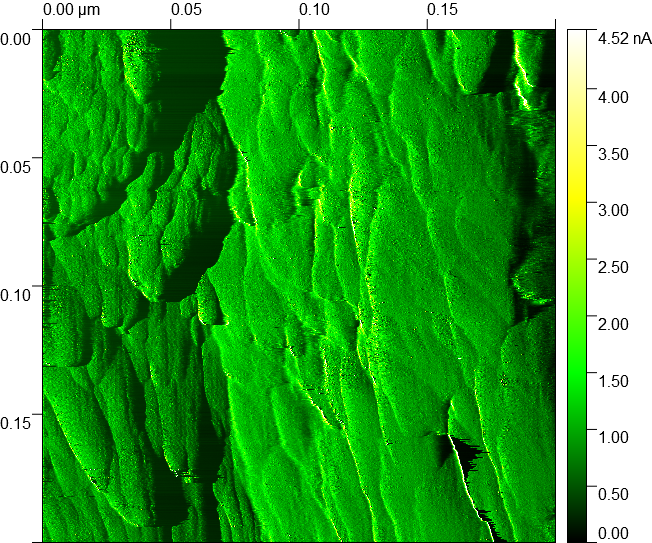
\includegraphics[width=\textwidth]{Au_Ecke_useI.png}
        \label{fig:goldecke_I}
    \end{minipage}
    \hfill
    \begin{minipage}[t]{0.495\textwidth}
        \centering
        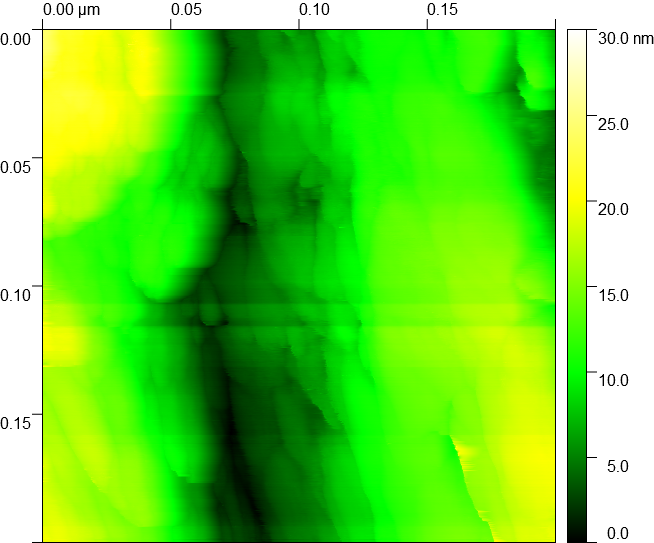
\includegraphics[width=\textwidth]{Au_Ecke_useZ.png}
        \label{fig:goldecke_Z}
    \end{minipage}
    \caption{
      RTM-Aufnahme Gold auf Silizium $\SI{200}{\nm}$; links: Tunnelstrom, rechts: Z-Achse; Setpoint $I = \SI{1}{\nano\ampere}$, Tip voltage $U = \SI{450}{\milli\volt}$,Rastergeschwindigkeit $v = \SI{500}{\nano\meter\per\second}$; $P = 1000$, $I = 2000$, $D = 0$
}
    \label{fig:goldecke_combined}
\end{figure}

Wie zu sehen ist, zeigen die Bilder tatsächlich eine raue Oberflächenstruktur in \cref{fig:goldecke_combined} und eine vergleichsweise glattere Oberflächenstruktur in \cref{fig:goldrund_combined}. 
In \cref{fig:goldecke_combined} deuten die starken Farbvariationen, die hier Höhenunterschiede repräsentieren, auf eine relativ rauere Oberfläche hin im Vergleich zu den schwachen Farbvariationen in \cref{fig:goldrund_combined}.


Dies spiegelt jedoch nicht notwendigerweise tatsächliche Höhenunterschiede in der Oberflächenstruktur wider, da das STM lediglich die Oberflächenladungsdichte detektiert und diese mit einer Höhe verknüpft. 
Da Gold ein Leiter ist, in dem sich Elektronen frei bewegen können, ist diese Verknüpfung nicht zwangsläufig physikalisch sinnvoll (bei metallischen Oberflächen Elektronendichte und wirkliche Topografie schwer zu trennen sind, da die Elektronen delokalisiert sind).

Wie zu erwarten stimmt die Gesamtstruktur des Materials (Sowohl \cref{fig:goldrund_combined} als auch \cref{fig:goldecke_combined}) sehr mit den in der Praktikumsanleitung \cite{praktikum} bereitgestellten Bildern überein.
Zudem sind wolkenartige Strukturen erkennbar, die, wie erwartet, das verdampfte Gold repräsentieren. 
Das Bild erscheint gelungen, da auf der rechten Seite nur eine scharfe Kante sichtbar ist, die höchstwahrscheinlich natürlichen Ursprungs und nicht auf eine unpräzise Oberflächenabtastung zurückzuführen ist. 
Ein Hinweis darauf ist, dass unter dem USB-Mikroskop bereits Kratzer im Mikrometerbereich beobachtet wurden, die in derselben Größenordnung wie der $\SI{2}{\micro\metre} \times \SI{2}{\micro\metre}$ Bildausschnitt liegen. 
Es ist daher wahrscheinlich, dass kleinere Kratzer ähnlicher Größe existieren, die mit dem USB-Mikroskop nicht sichtbar waren.


Bei \cref{fig:goldecke_combined} sind die Farbvariationen vergleichsweise minimal, und die wenigen Anomalien lassen sich auf Kratzer und zerbrochene Segmente zurückführen, die aufgrund der begrenzten Auflösung des USB-Mikroskops zu klein sind, um eindeutig dargestellt zu werden.


Da das STM bei Gold ohne Absturz arbeitete und repräsentative Topografien lieferte, folgt nun die Untersuchung der anspruchsvolleren HOPG-Probe.
